\documentclass{standalone}
\usepackage{tkz-base}
\usepackage{tkz-fct}
\usepackage{tkz-euclide}
\usepackage{tikz}
\begin{document}
    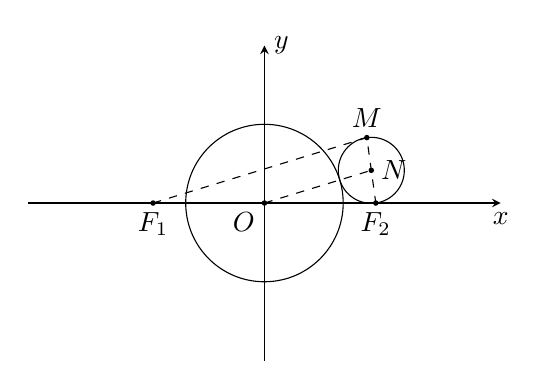
\begin{tikzpicture}
        \pgfmathsetmacro\xx{3}
        \pgfmathsetmacro\y{2}
        \pgfmathsetmacro\a{1}
        \pgfmathsetmacro\b{1}
        \pgfmathsetmacro\c{sqrt(abs(\a^2+\b^2))}
        \pgfmathsetmacro\px{1.3}
        \pgfmathsetmacro\py{sqrt(-1*\b^2*(1-(\px^2)/\a^2))}
        \coordinate (O) at (0,0);
        \coordinate (F1) at (-\c,0);
        \coordinate (F2) at (\c,0);
        \coordinate (M) at (\px,\py);
        \coordinate (N) at ($(M)!0.5!(F2)$);
        \pgfmathsetmacro\rN{sqrt((\px-\c)^2+\py^2)/2}
        \tkzInit[ymax=\y,ymin=-\y,xmax=\xx,xmin=-\xx] 
        % \tkzGrid
        % \tkzDrawXY[noticks,-stealth]
        \tkzFctPar[samples=400,domain=-0.4*pi:0.4*pi]{\a/(cos(t))}{\b*(tan(t))}
        \tkzFctPar[samples=400,domain=0.6*pi:1.4*pi]{\a/(cos(t))}{\b*(tan(t))}
        \draw[-stealth] (-\xx,0) -- (\xx,0) node [below] {$x$};
        \draw[-stealth] (0,-\y) -- (0,\y) node [right] {$y$};
        \fill (O) node [below left] {$O$} circle (1pt);
        \fill (F1) node [below] {$F_1$} circle (1pt);
        \fill (F2) node [below] {$F_2$} circle (1pt);
        \fill (M) node [above] {$M$} circle (1pt);
        \fill (N) node [right] {$N$} circle (1pt);
        \draw (O) circle (\a);
        \draw (N) circle (\rN);
        \draw[dashed] (F1) -- (M) -- (F2) (O)--(N);
    \end{tikzpicture}
\end{document}